\chapter{SysCo manipulation}
\label{Chap:SysCo}


%-----------------------------------------------------------------------
%-----------------------------------------------------------------------
%-----------------------------------------------------------------------

\section{Introduction}

Coordinate systems (\textbf{SysCo}) types supported by \CdPPP\ are:
\begin{itemize}
\item \textbf{Local}: any Euclidian frame, without any geolocalization or vertical direction knowledge
\item \textbf{GeoC}: geocentric coordinates
\item \textbf{LEuc}: a local Euclidian frame with an affine transformation into geocentric coordinates
\item \textbf{RTL}: a special case of \texttt{LEuc}, with the local frame defined by an origin point where Z is normal to ellipsoid and X is on East direction (see ~\ref{SysCoRTL})
\item \textbf{Proj}: any georeferenced system supported by the \href{https://proj.org}{PROJ} library
\end{itemize}

When SysCo is known, its definition is recorded into the file \texttt{CurSysCo.xml}, in \texttt{Ori} and \texttt{PointsMeasure} directories.

%This file can be copied into \texttt{MMVII-PhgrProj/SysCo/} with a short name to be used in next commands.
%Example: copy \texttt{CurSysCo.xml} as \texttt{MMVII-PhgrProj/SysCo/MyCRS.xml}, to be able to use \texttt{MyCRS} as a SysCo name.

\section{Setting SysCo}

\subsection{MMVII Commands}
There are several ways to declare a data SysCo:

\begin{itemize}
\item with \texttt{SysCo} option in \texttt{ImportOri} command that imports orientations into a declared SysCo
\item with \texttt{ChSys} option in \texttt{ImportGCP} command that declares or transforms ground coordinates on-the-fly
\item some import commands with an implicit SysCo, such as \texttt{ImportInitExtSens} that supposes that RPC are always in WGS84 geographical coordinates system in degrees
\item \texttt{OriChSysCo} and \texttt{GCPChSysCo} commands that transforms orientations and ground points from one SysCo into another
\end{itemize}

\subsection{SysCo definition}
\label{subsec:SysCoDef}
The SysCo definitions for \CdPPP\ commands can be:
\begin{itemize}
\item the name of a file in \CdPPP\ source subfolder \texttt{MMVII/MMVII-RessourceDir/SysCo} or in project subfolder \texttt{MMVII-PhgrProj/SysCo}, without its extension, only its basename (e.g., \texttt{RTL} for \texttt{MMVII-PhgrProj/SysCo/RTL.xml} file)
\item any \texttt{PROJ} definition (e.g., \texttt{IGNF:LAMB93}, \texttt{EPSG:4326} or \texttt{'+proj=merc +lat\_ts=56.5 +datum=WGS84'})
\item any string starting with \texttt{Local} for a local frame (e.g., \texttt{LocalAMRules})
\item \texttt{GeoC} for a geocentric frame
\item a string starting with \texttt{LEuc}, with the pattern: \texttt{LEuc*TX*TY*TZ*Omega*Phi*Kappa}, where the transformation is given in geocentric coordinates, angles in rad
\item a string starting with \texttt{RTL}, with the pattern: \texttt{RTL*X0*Y0*Z0*Def} (e.g., \texttt{RTL*0.675*45.189*0*EPSG:4326}),
where you give the origin point coordinates in a certain PROJ system. Tip: use \texttt{SysCoCreateRTL} command to make it automatically (see ~\ref{SysCoRTL})

\end{itemize}


\subsection{Examples}
\begin{itemize}
\item \texttt{SysCo=L93} will set the SysCo to Lambert93 (IGNF:LAMB93), as defined in \\
\texttt{MMVII/MMVII-RessourceDir/SysCo/L93.xml}
\item \texttt{SysCo=IGNF:LAMB1} will set the SysCo to Lambert I
\item \texttt{SysCo=LocalPanel} will set the SysCo to a local frame defined as "LocalPanel", that will not be convertible into any other SysCo
\item \texttt{SysCo=RTL*657700*6860700*0*IGNF:LAMB93*} will set the SysCo to a tangent local Euclidian frame, with origin ($657700, 6860700, 0$) in Lambert 93
\item \texttt{SysCo=GeoC} will set the SysCo to geocentric coordinates
\item \texttt{SysCo=AMRealm} will use a project-defined SysCo if \texttt{MMVII-PhgrProj/SysCo/AMRealm.xml} exists. If not, "AMRealm" will be used as a PROJ definition, and an error will occur

\end{itemize}


\section{RTL SysCo}
\label{SysCoRTL}

\begin{figure}[h!]
\centering
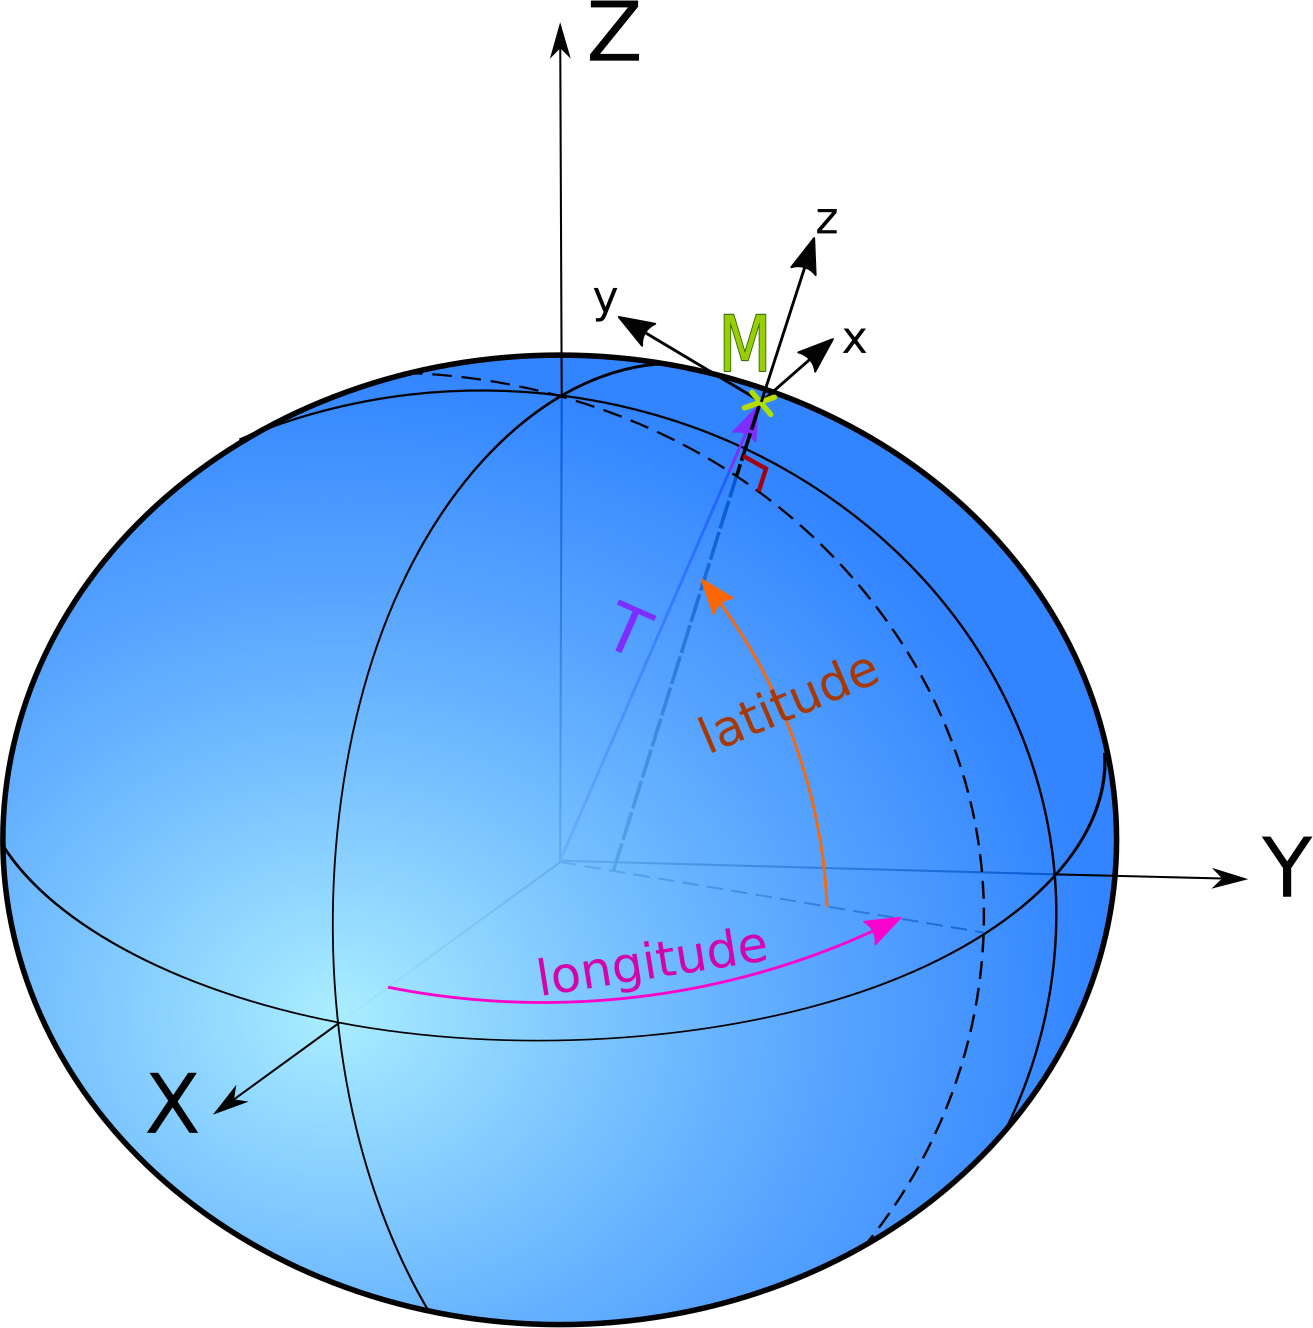
\includegraphics[width=9cm]{CommandReferences/ImagesComRef/cart_geocentr.png}
\caption{Local tangent frame (RTL) SysCo}
\label{fig:RTL}
\end{figure}


\CdPPP\ supposes that the coordinates used during bundle adjustment are Euclidian.

A local tangent frame (RTL) can be defined to simplify ones life. 

\texttt{SysCoCreateRTL} command does that from orientations, with the origin point being defined as the average of camera positions or a fixed point.

It creates a file with the chosen name in \texttt{MMVII-PhgrProj/SysCo/}.

Then every Ori and GCP is transformed into this RTL frame to be able to keep maximal precision during bundle adjustment.


\section{Testing transformation and PROJ installation}
The \texttt{TestProj} command is used to display PROJ log for a transformation between two SysCo.

\begin{verbatim}
 == Mandatory unnamed args : ==
  * string :: Input SysCo definition
  * string :: Output SysCo definition

 == Optional named args : ==
  * [Name=TestPoint] cPtxd<double,3> :: Point in input SysCo to check transformation
\end{verbatim}

Usage example: testing if we can safely convert from ellipsoid height into altitude
(from \texttt{IGNF:LAMB93} into \texttt{EPSG:5698}, meaning RGF93 v1/Lambert-93 + NGF-IGN69 height):

\begin{verbatim}
MMVII TestProj "L93" "EPSG:5698" TestPoint=[657723,6860710,0]

    PROJ LOG: pj_open_lib(proj.db): call fopen(/usr/share/proj/proj.db) - succeeded
    PROJ LOG: pj_open_lib(proj.ini): call fopen(/usr/share/proj/proj.ini) - succeeded
    Proj "+proj=geocent" to "+proj=latlong" accuracy: 0
    Proj "IGNF:LAMB93" to "+proj=geocent" accuracy: 1
    PROJ LOG: pj_open_lib(proj.db): call fopen(/usr/share/proj/proj.db) - succeeded
    PROJ LOG: pj_open_lib(proj.ini): call fopen(/usr/share/proj/proj.ini) - succeeded
    Proj "+proj=geocent" to "+proj=latlong" accuracy: 0
    PROJ LOG: pj_open_lib(fr_ign_RAF18.tif): call fopen(fr_ign_RAF18.tif) - failed
    PROJ LOG: pj_open_lib(RAF18.gtx): call fopen(RAF18.gtx) - failed
    PROJ LOG: pj_open_lib(fr_ign_RAF20.tif): call fopen(fr_ign_RAF20.tif) - failed
    PROJ LOG: pj_open_lib(fr_2019m.asc): call fopen(fr_2019m.asc) - failed
    PROJ LOG: pj_open_lib(fr_2019z.asc): call fopen(fr_2019z.asc) - failed
    Proj "EPSG:5698" to "+proj=geocent" accuracy: -1
                    SysIn                 =>                 SysOut                
    [657723.00000,6860710.00000,0.00000]  =>  [657723.00000,6860710.00000,-0.00000]
\end{verbatim}

Here, for the \texttt{TestPoint}, the output altitude is equal to the height, which in fact should be $-43.77823$.
The PROJ log messages show that the RAF grids are missing, hence the error.

See ~\ref{ProjData} for PROJ additional data installation.


\section{Proj additional data}
\label{ProjData}
Additional data for PROJ can be downloaded here: \url{https://download.osgeo.org/proj/}.

On GNU/Linux, it should be copied into $\sim$\texttt{/.local/share/proj/}.

On Windows, it should be copied into \texttt{MMVII\textbackslash share\textbackslash proj\textbackslash}.



%-----------------------------------------------------------------------
%-----------------------------------------------------------------------
%-----------------------------------------------------------------------

\chapter{Survey compensation}
\label{Chap:TopoUser}

\section{Survey introduction}

In \CdPPP, it is possible to add topographic survey measurements in global adjustments, alongside photogrammetric measurements. From now on, for convenience, "topo" term will be used instead of "topographic survey".

Topo measurements are made from an instrument that is verticalized/plumb or not.
The position and orientation of an instrument define a \textit{station}.
All the measurements are attached to a station and are expressed in the station frame (Fig. \ref{fig:topoStation}).

\begin{figure}[!h]
\centering
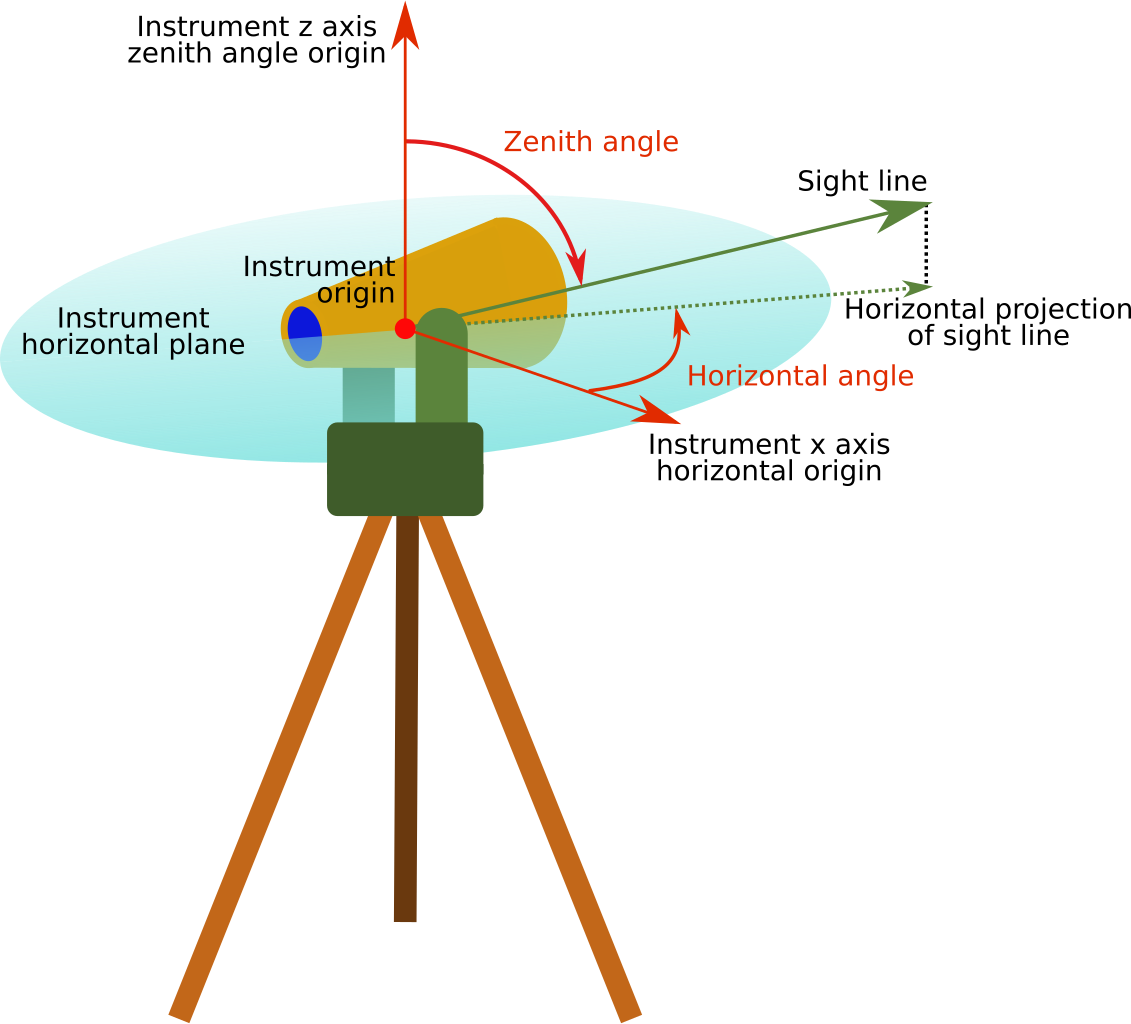
\includegraphics[width=9cm]{CommandReferences/ImagesComRef/topo.png}
\caption{A topo station, its frame and measured angles}
\label{fig:topoStation}
\end{figure}

The following measurements types are currently supported:

\begin{itemize}
    \item distances
    \item horizontal angles
    \item zenithal angles
    \item direct Euclidian vector observation
\end{itemize}

The measurements can be made between cameras poses, GCPs or undeclared points that will be inserted into the last GCP set of the adjustment
(if automatic coordinates initialization succeeds).

Two \CdPPP\ commands can use topo measurements in compensation:
\begin{itemize}
    \item \texttt{OriBundleAdj} via the \texttt{TopoFile} option
    \item \texttt{TopoAdj} (see \ref{subsec:TopoAdj})
\end{itemize}

The topo measurements files can be given as a set of \CdPPP\ json or xml files, or in a simplified text format (named \texttt{OBS} file) inherited from IGN's
Comp3D\footnote{\url{https://github.com/IGNF/Comp3D}} micro-geodesy compensation software.

All the measurements files must be in the \texttt{MMVII-PhgrProj/Topo/[TopoObsName]} folder.

\section{\texttt{OBS} file format}
\label{sec:compObsFormat}

Note: \CdPPP\ supports only a subset of Comp3D \texttt{OBS} format\footnote{\url{https://ignf.github.io/Comp3D/doc/obs.html}}.

\texttt{OBS} files are text files with fields delimited by any number of spaces or tabs. Blank lines are overlooked.
The \texttt{*} character defines a comment that goes up to the end of the line.

A measurement line is composed by:

\begin{itemize}
    \item code: an integer representing the type of observation (see below)
    \item station name
    \item target name
    \item measurement value (in meters for distances, in gon for angles)
    \item measurement \textit{a priori} $\sigma$ (in meters for distances, in gon for angles)
    \item anything else is ignored until the end of the line
\end{itemize}

Example of an \texttt{OBS} line describing a measured distance of 100.0000 m, with a $\sigma$ of 1 mm from \texttt{PointA} to \texttt{PointB}:

\begin{verbatim}
    3   PointA    PointB    100.0000    0.001    * comment
\end{verbatim}

The observations codes are:

\begin{itemize}
    \item \textbf{3}: 3D distance
    \item \textbf{5}: local horizontal (hz) angle
    \item \textbf{6}: local zenithal (zen) angle
    \item \textbf{7}: local horizontal angle for a new station 
    \item \textbf{14}: local $\Delta$x
    \item \textbf{15}: local $\Delta$y
    \item \textbf{16}: local $\Delta$z
\end{itemize}

\newpage
\section{Quickstart example}

An example of topo dataset can be found in \texttt{MMVII/MMVII-UseCaseDataSet/TopoMini/}.
It corresponds to this configuration:

\begin{figure}[!h]
\centering
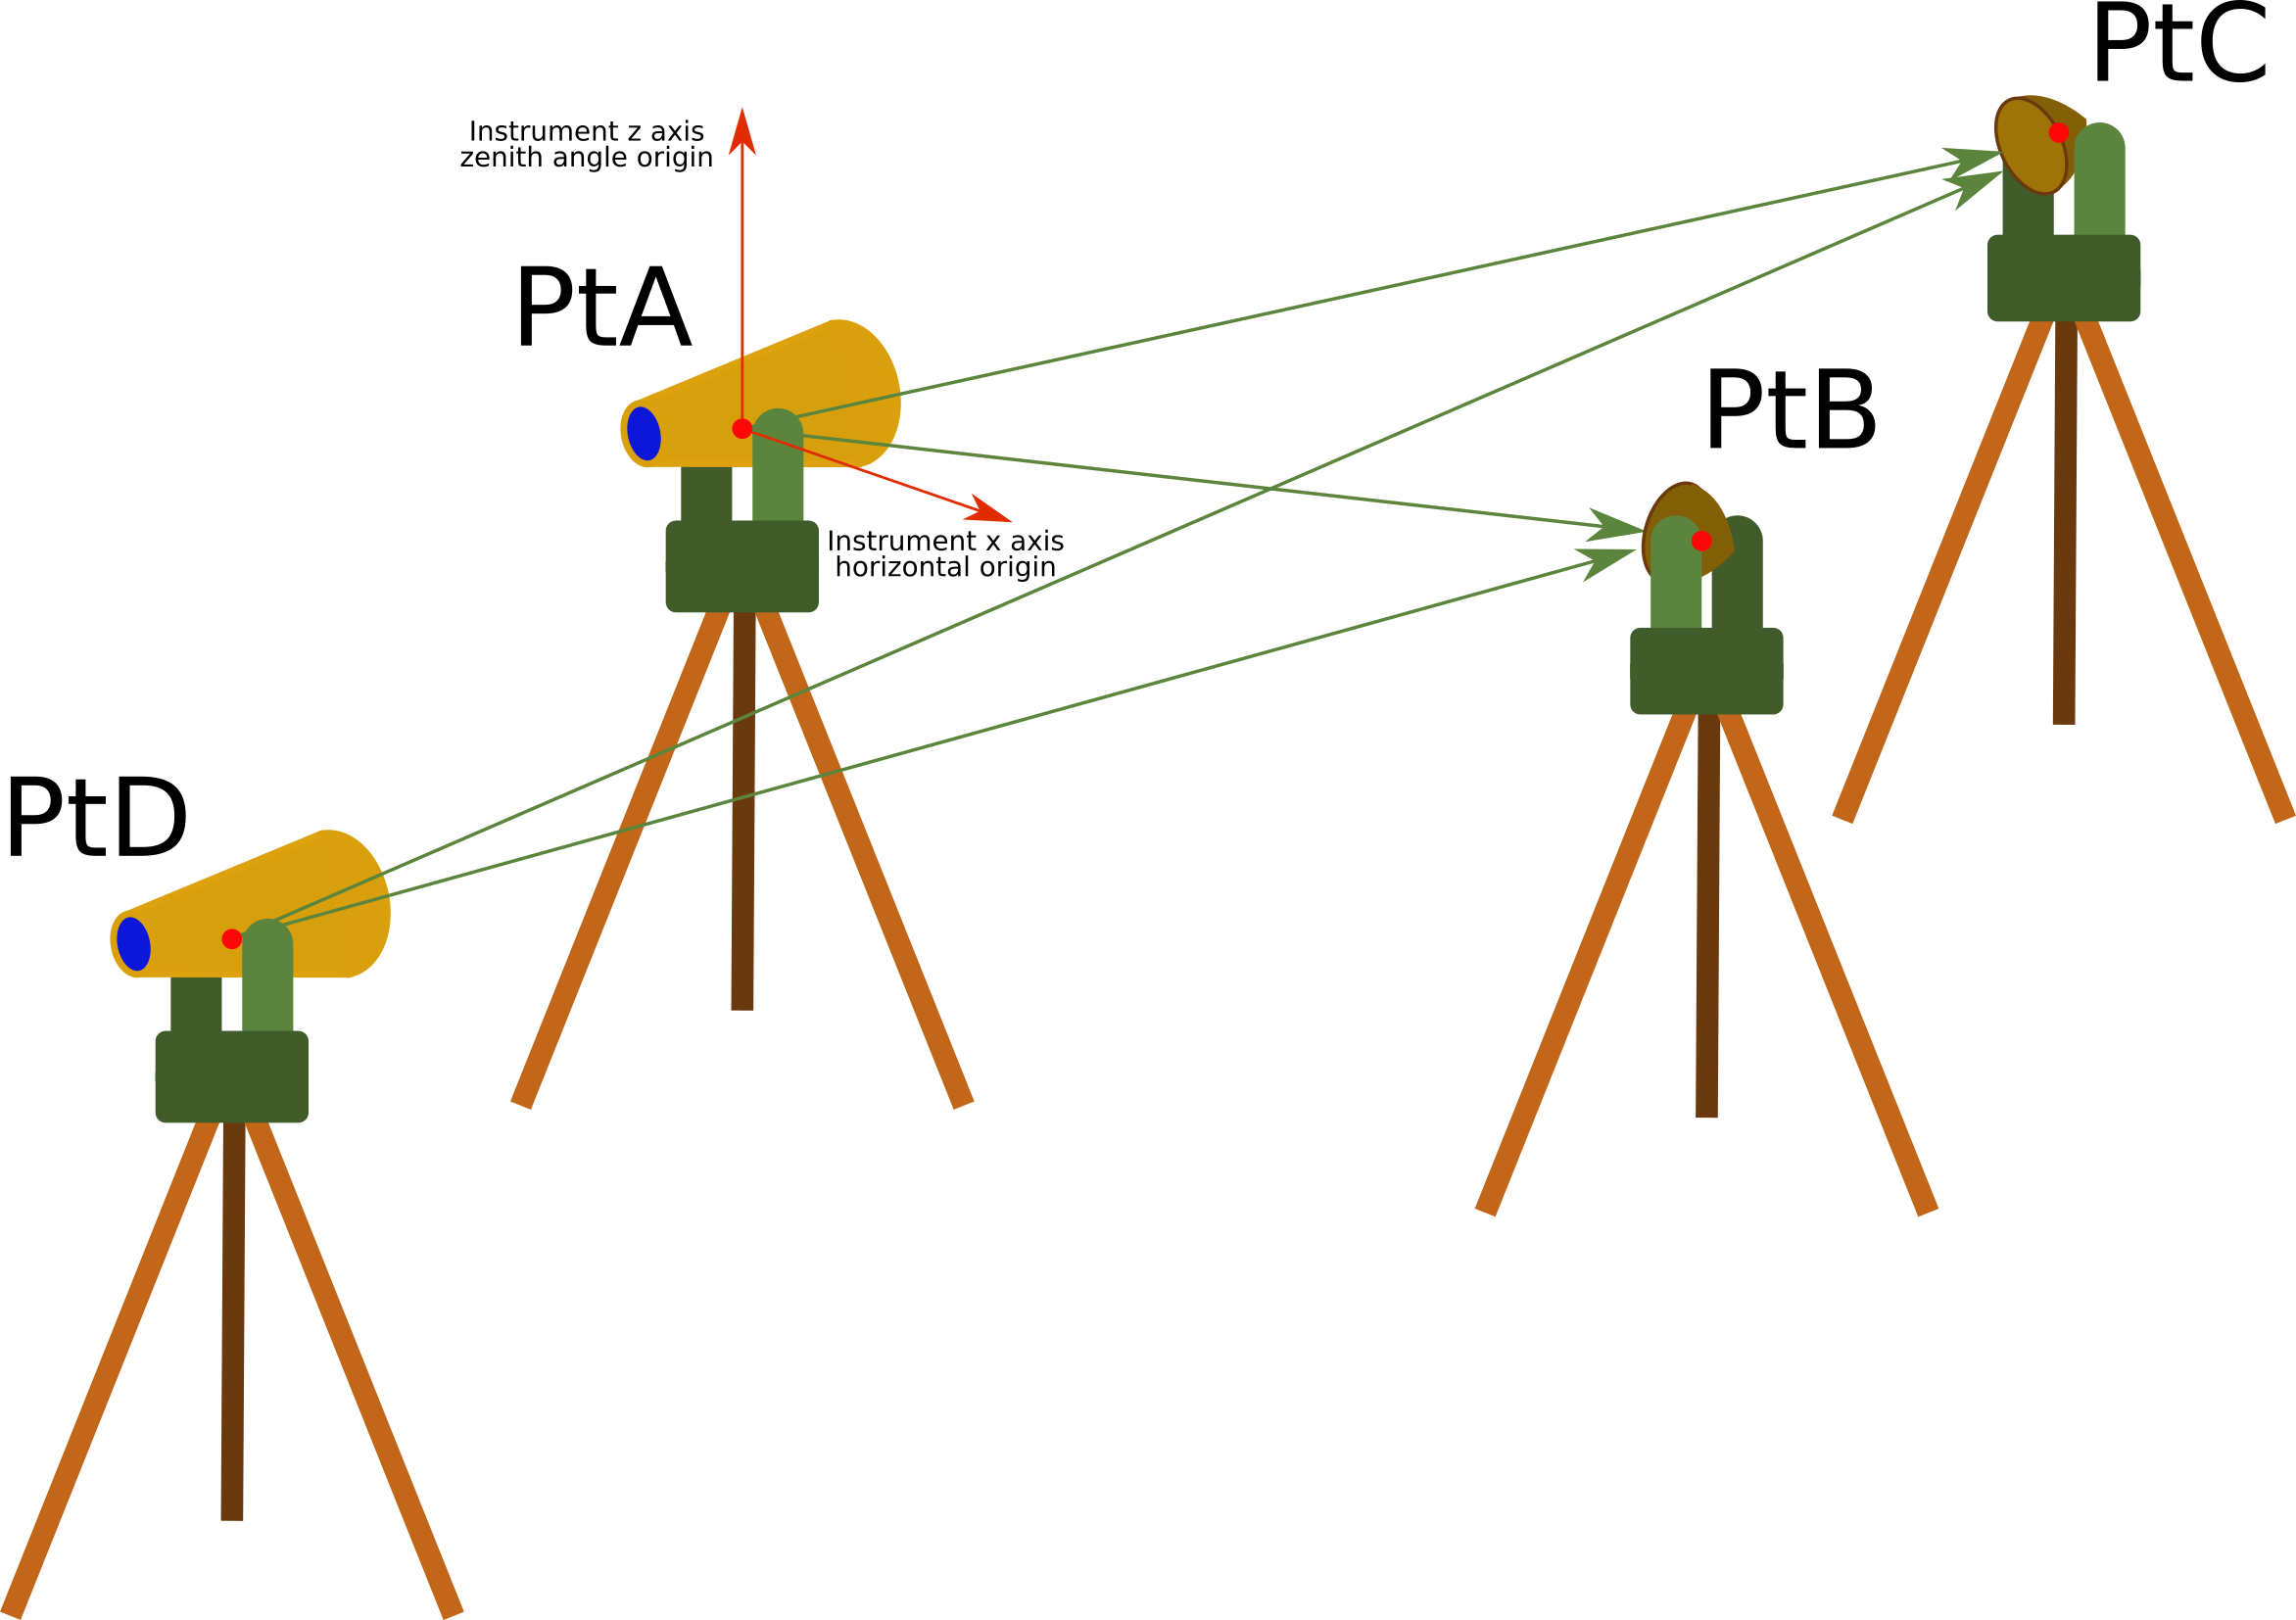
\includegraphics[width=11cm]{CommandReferences/ImagesComRef/topo2.png}
\caption{The \texttt{TopoMini} dataset}
\label{fig:topoSurvey}
\end{figure}

% PtA and PtD have known coordinates, PtB and PtC coordinates have to be computed (only approximate coordinates are known for this two points).

\subsection{3D points file}
The initial coordinates of the 4 points, in Lambert 93, are in a simple text file (\texttt{inputs/coords.txt}):

\begin{verbatim}
* 1st column:  0 = free point
1  PtA  657700.000  6860700.000  10.000
0  PtB  657710      6860700      10   * approx
0  PtC  657710      6860710      10   * approx
1  PtD  657700.000  6860690.000  10.000
\end{verbatim}

The coordinates of PtA and PtD are supposed known (with a certain precision).
The coordinates of PtB and PtC are just for initialization.
\\

To import these coordinates in \CdPPP\ we use the \texttt{ImportGCP} command, where we give the text format
(additional\_info, name, x, y, z), the name of the resulting \texttt{PointsMeasure} and the coordinates SysCo.
We also specify that the points that have '0' for their additional\_info are free points, that the sigma for
known points is 0.001m and that lines starting with '*' are comment lines.

\begin{lstlisting}
MMVII ImportGCP inputs/coords.txt ANXYZ InitL93 ChSys=[L93] AddInfoFree=0 Sigma=0.001 Comment=*
\end{lstlisting}

In the resulting file \texttt{MMVII-PhgrProj/PointsMeasure/InitL93/MesGCP-coords.xml},
the points PtA and PtD have a set \texttt{\_\_Opt\_\_Sigma2} equivalent to $\sigma = 0.001 m$ ,
the points PtB and PtC have no \texttt{\_\_Opt\_\_Sigma2}, making them free points.


\subsection{SysCo}

A \texttt{RTL} SysCo is mandatory to be able to compute a topo compensation.
PtA is chosen as RTL origin (tangency point).
The SysCo definition according to \ref{subsec:SysCoDef} is: \texttt{RTL*657700*6860700*0*IGNF:LAMB93}.
The \texttt{GCPChSysCo} command does the conversion to \texttt{RTL}:

\begin{lstlisting}
MMVII GCPChSysCo "RTL*657700*6860700*0*IGNF:LAMB93" InitL93 InitRTL
\end{lstlisting}

\begin{comment}
\subsection{SysCo shortcut}
The SysCo file \texttt{MMVII-PhgrProj/PointsMeasure/InitRTL/CurSysCo.xml}, created by \texttt{ImportGCP}
can be used to create a shortcut name for \texttt{RTL*657700*6860700*0*IGNF:LAMB93}.

We just have to copy it as \texttt{MMVII-PhgrProj/SysCo/RTL.xml} to be able to designate this SysCo
simply as \texttt{RTL} for the rest of the example.

\begin{lstlisting}
cp MMVII-PhgrProj/PointsMeasure/InitRTL/CurSysCo.xml MMVII-PhgrProj/SysCo/RTL.xml
\end{lstlisting}
\end{comment}


\subsection{Measurements}
The measurements are:
\begin{itemize}
   \item an instrument on PtA measures hz angle, zen angle and distance to PtB and PtC
   \item an instrument on PtD measures hz angle, zen angle and distance to PtB and PtC
\end{itemize}
The corresponding \texttt{OBS} file (\texttt{inputs/meas.obs}) is:
\begin{verbatim}
 7   PtA    PtB     0      0.001
 6   PtA    PtB   100      0.001
 3   PtA    PtB    10.05   0.005
 5   PtA    PtC   -40.62   0.001
 6   PtA    PtC   100      0.001
 3   PtA    PtC    14.88   0.005

 7   PtD    PtB     0      0.001
 6   PtD    PtB   100      0.001
 3   PtD    PtB    14.88   0.005
 5   PtD    PtC   -14.96   0.001
 6   PtD    PtC   100      0.001
 3   PtD    PtC    22.82   0.005
\end{verbatim}
This file has to be copied into a subdirectory of \texttt{MMVII-PhgrProj/Topo}:
\begin{lstlisting}
mkdir -p MMVII-PhgrProj/Topo/Obs1/
cp inputs/meas.obs MMVII-PhgrProj/Topo/Obs1/
\end{lstlisting}


\subsection{Unknowns count}

The previous \texttt{OBS} file creates two verticalized stations, one with its origin on PtA, the other on PtD.
Each of these stations has an horizontal orientation unknown ($G_0$) due to the random orientation of the instrument
when it has been set on the point.

The number of unknowns in this configuration is:
\begin{itemize}
   \item 3 per point ($x, y, z$)  $\rightarrow$ \textit{12 unknowns}
   \item 1 per station ($G_0$)  $\rightarrow$ \textit{2 unknowns}
\end{itemize}

Which gives a total of 14 unknowns for the 4 points and 2 stations.
% Total: $4 \times 3 + 2 \times 1 = 14$ unknowns.
\\

The number of constraints is:
\begin{itemize}
   \item 3 per constrained point, PtA and PtD  $\rightarrow$ \textit{6 constraints}
   \item 1 per topo measurement $\rightarrow$ \textit{12 constraints}
\end{itemize}

Which gives a total of 18 constraints.
% Total: $2 \times 3 + 12 = 18$ constraints.


\subsection{Adjustment}
\label{subsec:TopoAdj}
The \texttt{TopoAdj} command can perform an adjustment between topo and GCP constraints.
It is used as a substitute to \texttt{OriBundleAdj} when there are no cameras.

\begin{verbatim}
 == Mandatory unnamed args : ==
  * string [Topo,In] :: Dir for Topo measures
  * string [Topo,Out] :: Dir for Topo measures output
  * string [PointsMeasure,In] :: Dir for points initial coordinates
  * string [PointsMeasure,Out] :: Dir for points final coordinates

 == Optional named args : ==
  * [Name=GCPW] double :: Constrained GCP weight factor (default: 1)
  * [Name=DataDir] string :: Default data directories  ,[Default=Std]
  * [Name=NbIter] int :: Number of iterations ,[Default=10]
  * [Name=GCPFilter] string :: Pattern to filter GCP by name
  * [Name=GCPFilterAdd] string :: Pattern to filter GCP by additional info
  * [Name=GCPDirOut] string [PointsMeasure,Out] :: Dir for output GCP
  * [Name=LVM] double :: Levenberg–Marquardt parameter (to have better conditioning
                         of least squares) ,[Default=0]
\end{verbatim}

In our example, the input topo directory is \texttt{Obs1} and the input PointsMeasure is \texttt{InitRTL}.
We give output directories names for topo and points.
\begin{lstlisting}
MMVII TopoAdj Obs1 Obs1_out InitRTL FinalRTL
\end{lstlisting}

The final $\sigma_0$ value should be around 1 if everything goes well.
In this example, $\sigma_{0 init} > 5000$, because the initial coordinates of PtB and PtC are approximate,
and after 10 iterations it stabilizes at $\sigma_{0 final} = 1.7$.
\\

The output topo directory contains a single xml file with all the measurements and some output values (residuals,
stations orientations...). It can be used as topo input file.
\\

The last step is to convert the RTL coordinates to Lambert 93:

\begin{lstlisting}
MMVII GCPChSysCo L93 FinalRTL FinalL93
\end{lstlisting}


\section{Stations orientation constraints}

Each station has orientation constraints that have to be given before the station observations lines in the \texttt{OBS} file.
Each orientation constraint is indicated as a line starting with \texttt{\#} (from now on, called a \texttt{\#}-line).
\\

The possible orientation constraints are:
\begin{itemize}
   \item \texttt{\#FIX}: the station is axis-aligned, it is verticalized and oriented to North
   \item \texttt{\#VERT}: the station is verticalized and only horizontal orientation is free
   \item \texttt{\#BASC}: the station orientation has 3 degrees of freedom, meaning non-verticalized and not oriented to North
   \item TODO \texttt{\#CAM}:the station orientation is the camera orientation (only allowed for point names that correspond to image file names)
\end{itemize}

After a \texttt{\#}-line, all the following stations have the new orientation constraint until the next \texttt{\#}-line with new orientation unknowns.
For convenience, \texttt{\#NEW} can be used to keep current orientation constraint type and just add new unknowns for orientation (see \ref{subsec:SeveralStationsSamePoint}).


Each \texttt{OBS} file starts with an implicit \texttt{\#VERT}, making the stations verticalized by default.

For now, the vertical is modeled as the Earth's ellipsoid normal. Vertical deflection grids may be added later.



\subsection{Frames for survey stations}

The computation must take place in a 3D euclidian frame. For now, only RTL SysCo is supported.
Figure \ref{fig:topoFrames} shows the frames used in topo compensation.

\begin{figure}[!h]
\centering
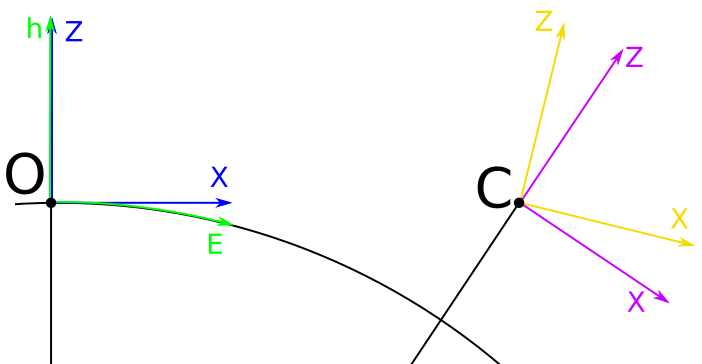
\includegraphics[width=12cm]{Programmer/framesTopo.png}
\caption{The different frames types used in compensation:
   \texttt{Green}: a projection SysCo. As it is not euclidian, compensation should not be done in this frame.
   \texttt{Blue}: the RTL SysCo for the computation. Every parameter is in this frame.
   \texttt{Purple}: each 3D point has its own local euclidian frame tangent to the ellipsoid
   \texttt{Yellow}: each topometric station has a rotation between the local euclidian tangent frame and the instrument frame.
 }
\label{fig:topoFrames}
\end{figure}


Stations orientation constraints fix some parts of the rotation between local tangent frame and instrument frame:
no rotation (\textbf{\#FIX}), rotation around $Z$ only (\textbf{\#VERT}), or free rotation (\textbf{\#BASC}).



\subsection{Return to quickstart example}
The example \texttt{OBS} file was:
\begin{verbatim}
 7   PtA    PtB     0      0.001
 6   PtA    PtB   100      0.001
 3   PtA    PtB    10.05   0.005
 5   PtA    PtC   -40.62   0.001
 6   PtA    PtC   100      0.001
 3   PtA    PtC    14.88   0.005

 7   PtD    PtB     0      0.001
 6   PtD    PtB   100      0.001
 3   PtD    PtB    14.88   0.005
 5   PtD    PtC   -14.96   0.001
 6   PtD    PtC   100      0.001
 3   PtD    PtC    22.82   0.005
\end{verbatim}

It is possible to say that the station on PtA was not verticalized by using \texttt{\#BASC}:
\begin{verbatim}
#BASC
 7   PtA    PtB     0      0.001
 6   PtA    PtB   100      0.001
 3   PtA    PtB    10.05   0.005
 5   PtA    PtC   -40.62   0.001
 6   PtA    PtC   100      0.001
 3   PtA    PtC    14.88   0.005

#VERT
 7   PtD    PtB     0      0.001
 6   PtD    PtB   100      0.001
 3   PtD    PtB    14.88   0.005
 5   PtD    PtC   -14.96   0.001
 6   PtD    PtC   100      0.001
 3   PtD    PtC    22.82   0.005
\end{verbatim}

This will free the 3D rotation of the station on PtA, adding two rotations unknowns to the computation.
\newline

It is also possible to use \texttt{\#FIX} to remove the horizontal orientation unknown $G_0$ of a station, expressing the fact that it
is verticalized and the horizontal reference is North:
\begin{verbatim}
#FIX
 7   PtA    PtB     0      0.001
 6   PtA    PtB   100      0.001
 3   PtA    PtB    10.05   0.005
 5   PtA    PtC   -40.62   0.001
 6   PtA    PtC   100      0.001
 3   PtA    PtC    14.88   0.005

#VERT
 7   PtD    PtB     0      0.001
 6   PtD    PtB   100      0.001
 3   PtD    PtB    14.88   0.005
 5   PtD    PtC   -14.96   0.001
 6   PtD    PtC   100      0.001
 3   PtD    PtC    22.82   0.005
\end{verbatim}


\subsection{Several stations on the same point}
\label{subsec:SeveralStationsSamePoint}

\CdPPP\ automatically creates a new station when a point is used for the first time as the origin of a measurement.

If we have to make a new set of orientation unknowns because two instruments were set on the same point with different
orientations, we can either:

\begin{itemize}
   \item use separate \texttt{OBS} files
   \item add a \texttt{\#}-line to separate the measurements sets (\texttt{\#NEW} is useful in this case to make a station with the same orientation constraints as before)
   \item use a code \textbf{7} instead of \textbf{5} for the first measurement of the new station
\end{itemize}

A separate \texttt{OBS} files or a \texttt{\#}-line closes all current stations.
Code \textbf{7} only closes the previous station on one point. 

Some illustrations :
\begin{verbatim}
 7   St1    PtA   100.000   0.001 * creates a station on St1
 5   St1    PtB   110.000   0.001

 7   St1    PtA   150.000   0.001 * closes current station on St1, creates a new one on St1
 5   St1    PtC   210.000   0.001
\end{verbatim}
Creates two stations originating on point \texttt{St1}. Each of these station
is vericalized (thanks to the implicit \texttt{\#VERT} at the start of the file) and each has one horizontal orientation unknown.
Here, there is a 50 grades difference between the two stations orientations.

With:
\begin{verbatim}
 7   St1    PtA     100.000      0.001 * creates a station on St1
 5   St1    PtB     110.000      0.001

 5   St1    PtA     150.000      0.001
 5   St1    PtC     210.000      0.001
\end{verbatim}
There is only one station on \texttt{St1}. The incoherent horizontal angles values
will make the computation fail.

Another way to fix it:
\begin{verbatim}
 5   St1    PtA     100.000      0.001 * creates a station on St1
 5   St1    PtB     110.000      0.001
#NEW                                   * closes all current stations
 5   St1    PtA     150.000      0.001 * creates a station on St1
 5   St1    PtC     210.000      0.001
\end{verbatim}
The fisrt \textbf{7} is not mandatory since it is the start of a file, there is no
current stations. \texttt{\#NEW} closes all the current stations, keeping the same orientations constraints (stations verticalized).

Code \textbf{7} only closes the current station on one point :
\begin{verbatim}
 5   St1    PtA   100.000   0.001 * creates a station on St1
 5   St1    PtB   110.000   0.001
 
 5   St2    PtA   200.000   0.001 * creates a station on St2
 5   St2    PtD   300.000   0.001

 7   St1    PtA   150.000   0.001 * closes station on St1, creates a new one on St1
 5   St1    PtC   210.000   0.001

 5   St2    PtE   250.000   0.001 * uses previous station on St2
\end{verbatim}
But:
\begin{verbatim}
 5   St1    PtA   100.000   0.001 * creates a station on St1
 5   St1    PtB   110.000   0.001
 
 5   St2    PtA   200.000   0.001 * creates a station on St2
 5   St2    PtD   300.000   0.001
#NEW                              * closes all the stations
 5   St1    PtA   150.000   0.001 * creates a station on St1
 5   St1    PtC   210.000   0.001

 5   St2    PtE   250.000   0.001 * creates a station on St2
\end{verbatim}


\subsection{Special case for distance-only measurements}

If a station only has distances measurements, it is automatically
set as a \texttt{\#FIX} station, since this station orientation unknowns
can't be estimated.


\section{Topo measurements for minimal external constraints}

For any kind of adjustment, minimal constraints can be useful to get the measurements internal precision.
In general, several GCP with known coordinates are used to fix the frame, but their inconsistency may
impact the computation.

In a 3D adjustment, up to 7 external constraints have to be provided to fix the frame translation, rotation ($R_X$, $R_Y$, $R_Z$) and scale.

With photogrammetry, one camera pose can be used to fix 6 external constraints. The scale can then be given with an \texttt{OBS} file:
\begin{verbatim}
    * distance of 10 meters between IMG1.JPG and IMG2.JPG poses centers
    3  IMG1.JPG  IMG2.JPG 10.0000 0.0010   
\end{verbatim}

Another possibility is to constrain the coordinates of one GCP, then add an \texttt{OBS} file to fix the scale and the 3 rotations:
\begin{verbatim}
    3  IMG1.JPG  IMG2.JPG 10.0000 0.0010   * scale constraint

    #FIX  * do not add a rotation unknown
    5  IMG1.JPG  GCP_10  0   0.0010   * GCP_10 is north from IMG1.JPG => constraints Rz

    * two Za=Zb constraints between non-aligned points to constrain Rx and Ry
    16  GCP_03  GCP_10  0 0.0010
    16  GCP_03  GCP_11  0 0.0010
\end{verbatim}

Minimal external constraints for the quickstart example means having constraints on only one point and this \texttt{OBS} file:

\begin{verbatim}
#FIX
 5   PtA    PtB   100      0.001 * PtA => PtB = East. Code 7 or 5 are equivalent here
 
#VERT
 7   PtA    PtB     0      0.001
 6   PtA    PtB   100      0.001
 3   PtA    PtB    10.05   0.005
 5   PtA    PtC   -40.62   0.001
 6   PtA    PtC   100      0.001
 3   PtA    PtC    14.88   0.005

 7   PtD    PtB     0      0.001
 6   PtD    PtB   100      0.001
 3   PtD    PtB    14.88   0.005
 5   PtD    PtC   -14.96   0.001
 6   PtD    PtC   100      0.001
 3   PtD    PtC    22.82   0.005
\end{verbatim}


\begin{comment}
\section{Topometric adjustment example}
\label{subsec:topoBench}

The example is used in \texttt{TopoComp} Bench. It is created by the method \texttt{cTopoData::createEx1()}.
We will describe the input files equivalent for the \texttt{TopoAdj} command.


\subsection{Creating the points}

The points with their initial coordinates and the sigmas on their coordinates constraints
are given in a GCP file. 

3 points have coordinates constraints at 1 cm ($A$, $B$, $C$). They form an isosceles triangle
on an horizontal plane.
A 4th point ($D$) is declared above the other. It has no \texttt{\_\_Opt\_\_Sigma2} attribute in the GCP file as this point is free.
(Fig. \ref{fig:topoEx1}). Note that depending on the initial coordinates for $D$, the computation may no succeed
(i.e., if $A$ and $D$ have the same initial coordinates, the distance formula derivatives are $NaN$).

A \texttt{CurSysCo.xml} must come along this GCP file to describe the RTL SysCo.


\begin{figure}[!h]
\centering
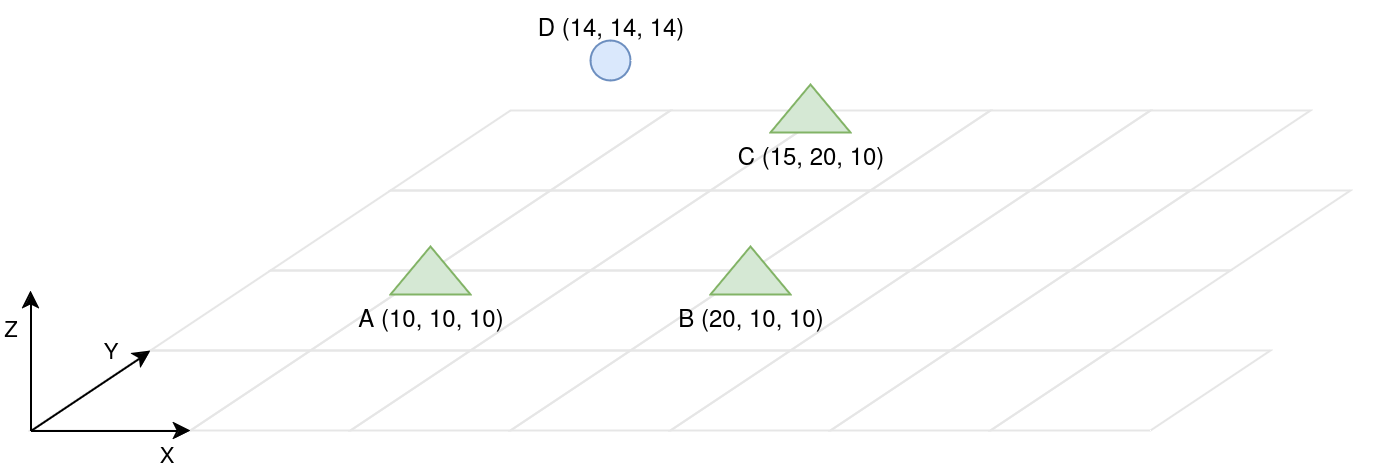
\includegraphics[width=12cm]{Programmer/benchtopo1b.png}
\caption{The 3 fixed points ($A$, $B$, $C$) and the free point ($D$)}
\label{fig:topoEx1}
\end{figure}

The summarized content of the GCP file:

\begin{lstlisting}
      <SetGCP>
         <NameSet>"terrain"</NameSet>
         <Measures>
            <el>
               <Name>"A"</Name>
               <Pt>10 10 10</Pt>
               <AdditionalInfo>""</AdditionalInfo>
               <__Opt__Sigma2>.0001 0 0 .0001 0 .0001</__Opt__Sigma2>
            </el>
            <el>
               <Name>"B"</Name>
               <Pt>20 10 10</Pt>
               <AdditionalInfo>""</AdditionalInfo>
               <__Opt__Sigma2>.0001 0 0 .0001 0 .0001</__Opt__Sigma2>
            </el>
            <el>
               <Name>"C"</Name>
               <Pt>15 20 10</Pt>
               <AdditionalInfo>""</AdditionalInfo>
               <__Opt__Sigma2>.0001 0 0 .0001 0 .0001</__Opt__Sigma2>
            </el>
            <el>
               <Name>"D"</Name>
               <Pt>14 14 14</Pt>
               <AdditionalInfo>""</AdditionalInfo>
            </el>
         </Measures>
      </SetGCP>
\end{lstlisting}


\subsection{Creating the observations}

The distances from $D$ to $A$, $B$ and $C$ are measured. For redundancy and error evaluation, the distance from $D$ to $C$ is measured twice
with different values (Fig. \ref{fig:topoEx2}).

\begin{figure}[!h]
\centering
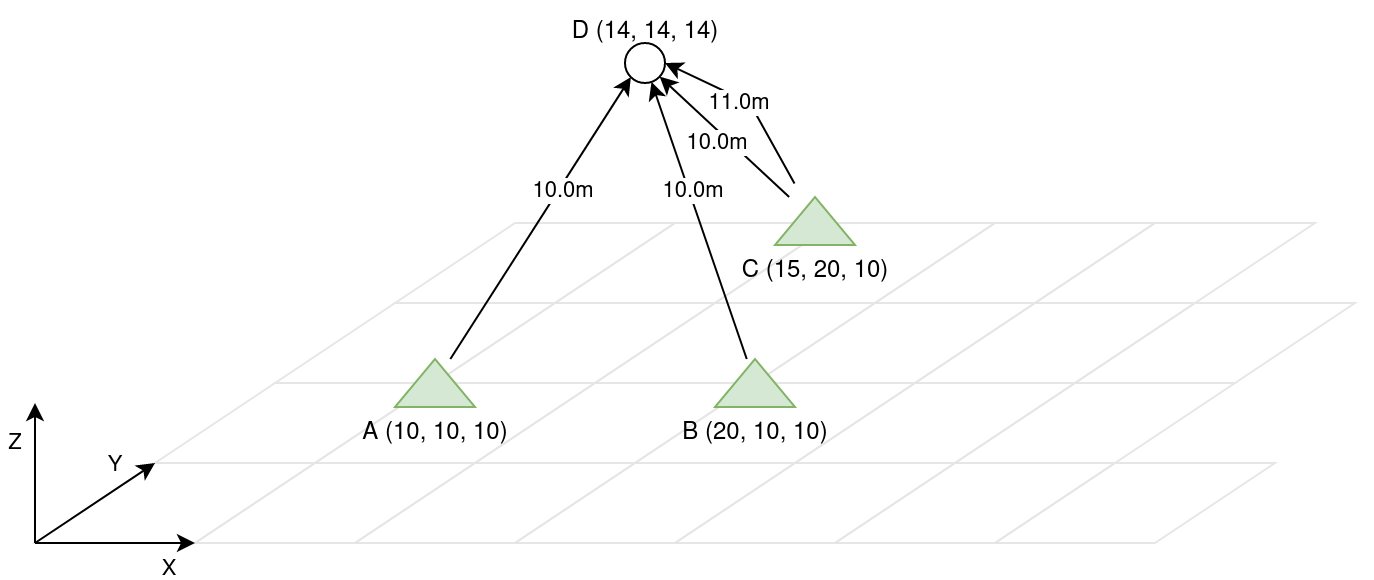
\includegraphics[width=12cm]{Programmer/benchtopo2.png}
\caption{Point $D$ is determined by measured distances}
\label{fig:topoEx2}
\end{figure}

Observations are represented in an \texttt{OBS} file:
\begin{lstlisting}
    3  D  A  10.0  0.1
    3  D  B  10.0  0.1
    3  D  C  10.0  0.1
    3  D  C  10.1  0.1
\end{lstlisting}

Here a implicit station is created, based on point $D$.
As no orientation status is given, the station is supposed verticalized.
It should have an horizontal orientation degree of liberty.
But since there is no observations able to determine the station orientation,
it is automatically set as fixed (as if a \texttt{\#FIX} line was added at the start of the file).

\subsection{Outputs}

After a computation, the output GCP file contains the final coordinates of every point, including
points that were not declared in the input GCP, but referenced in the topo measurements.

The output Topo file contains info about all the stations and observations,
with output values as residuals:

\begin{lstlisting}
<TopoData>
 <AllObsSetStations>
    <el>
       <TopoObsSetData>
          <Type>"Station"</Type>
          <AllObs>
             <el>
                <TopoObsData>
                   <Type>"Dist"</Type>
                   <Pts>    <el>"D"</el>     <el>"A"</el>       </Pts>
                   <Measures>    <el>10</el>      </Measures>
                   <Sigmas>   <el>0.1</el>     </Sigmas>
                   <__Opt__LastResiduals>  <el>-0.000000000000002</el>  </__Opt__LastResiduals>
                </TopoObsData>
             </el>
[...]
             <el>
                <TopoObsData>
                   <Type>"Dist"</Type>
                   <Pts>      <el>"D"</el>     <el>"C"</el>          </Pts>
                   <Measures>     <el>10.1</el>         </Measures>
                   <Sigmas>       <el>0.1</el>           </Sigmas>
                   <__Opt__LastResiduals>  <el>-0.050000000000001</el>  </__Opt__LastResiduals>
                </TopoObsData>
             </el>
          </AllObs>
          <StationOriStatus>"#FIX"</StationOriStatus>
          <__Opt__Out_G0>0</__Opt__Out_G0>
       </TopoObsSetData>
    </el>
 </AllObsSetStations>
</TopoData>
\end{lstlisting}

This Topo file can be used as input for another adjustment (it is completely equivalent to the \texttt{OBS} file).

\end{comment}
